\documentclass{article}
\usepackage{amsmath}
\usepackage{hyperref}
\usepackage{tikz}
\usetikzlibrary{arrows.meta}
\tikzset{
myptr/.style={-{Stealth[scale=2]}},
}
\begin{document}

\title{FM Demodulator SNR}
\maketitle

My take on an expression for FM demodulator SNR above threshold, based mainly on Carlson \cite{crilly2009communication} but also the noise triangle/phasor model discussed in various online and text sources.

Consider a FM signal $r(t)$ modulated by a sinusoidal message signal $x(t)$:
\begin{equation}
\begin{split}
r(t) &= A_c cos(2 \pi f_c t +\phi(t)) \\
\phi(t) &=  2 \pi f_d \int_0^t x(t) \\
x(t) &= A cos(2 \pi f_m t)
\end{split}
\end{equation}
where $A_c$ is the carrier level, $f_c$ the carrier frequency, $x(t)$ the message signal of peak amplitude $A \le 1$, and the peak deviation is $f_d$.  We assume we can extract the phase term $\phi(t)$ from the carrier phase $2 \pi f_c t$. An ideal FM demodulator can be modelled as: 
\begin{equation}
y(t) = \frac{d\phi}{dt}
\end{equation}
Giving the demodulated message signal:
\begin{equation}
\label{eq:fm_signal}
y_s(t) = 2 \pi f_d A cos (2 \pi f_m t)
\end{equation}
The average power at the demodulator output is then:
\begin{equation}
\label{eq:fm_signal_power}
S = (2 \pi f_d )^2 \frac{A^2}{2}
\end{equation}

\begin{figure}[h]
\begin{center}
\begin{tikzpicture}
\draw [myptr] (0,0) -- node[below] {$A_c$} (5,0);
\draw [myptr] (5,0) -- node[right] {$A_n$} (5,2);
\draw [myptr,blue] (0,0) -- (5,2);
\draw [myptr,dashed] (7,0) arc (0:360:2);
\node[above]  at (1.5,0) {$\phi_n$};
\node[left] at (7,0) {$f_n$};
\end{tikzpicture}
\end{center}
\caption{Phasor diagram showing the sum (blue) of the carrier signal with magnitude $A_c$ and a small noise vector of magnitude $A_n$.  Consider the noise vector to be a small slice of the input noise spectrum at frequency $f_n$ from the carrier. The noise vector rotates around the tip of the carrier vector at frequency $f_n$, creating sinusoidal modulation in $\phi_n$.}
\label{fig:phasor}
\end{figure}

Consider the FM carrier plus noise signal in Figure \ref{fig:phasor}.  As a thought experiment consider the signal has been frequency shifted such that the carrier frequency is now 0 and the carrier phasor lies stationary along the real axis.  The sum of the carrier and noise vector has variations in magnitude and phase, however our demodulator is only sensitive to changes in phase. Let $A_n$ be the magnitude of the signal from a small slice of the input noise spectrum, effectively a small interfering sine wave summed with the carrier. As the noise vector rotates, it generates a sinusoidally changing angle $\phi_n$.  The peak of the angle (deviation of the noise signal) occurs when $sin(\phi_n) = A_n/A_c$. For $A_c>>A_n$ we can use the approximation $\phi_n=A_n/A_c$.  By considering (\ref{eq:fm_signal}) the demodulated signal from the input noise at $f_c+f_n$ is:
\begin{equation}
\label{eq:fm_noise}
y_n(t) = 2 \pi f_n (A_n/A_c) cos(2 \pi f_n t)
\end{equation}
This is an interesting result:
\begin{enumerate}
\item The slice of noise at $f_c+f_n$ is demodulated as a baseband sine wave at $f_n$.
\item The amplitude of the demodulated noise is a function of $f_n$.
\end{enumerate}
This leads to the ``noise triangle" visualisation of FM where the noise is increasing as a function of frequency, unlike linear modulation scheme like SSB that have constant noise across frequency. The demodulator output power from the slice of noise at the demodulator input at frequency $f_c+f_n$ is:
\begin{equation}
\label{eq:fm_noise_power}
N(f_n) =  \frac{1}{2}(2 \pi f_n (A_n/A_c) )^2 
\end{equation}
The total noise power in the demodulator output is the noise power per unit bandwidth summed over the interval $[-f_m,f_m]$, where $f_m$ is the maximum frequency of the message signal $x(t)$. Using the 1:1 frequency relationship between a noise slice at the demodulator input and output (\ref{eq:fm_noise}), we can integrate (\ref{eq:fm_noise_power}) over the interval $[-f_m,f_m]$ to find the total noise power:
\begin{equation}
N = (2\pi)^2 \frac{N_0}{C} \int_{-f_m}^{f_m} f_n^2 df_n = (2\pi)^2 \frac{N_0}{3C} f_m^3
\end{equation}
where $N_0=A_n^2$ is the demodulator input power per unit bandwidth, and $C=A_c^2$ is the carrier power.  The signal to noise ratio at the FM demodulator output is then \cite{crilly2009communication}:
\begin{equation}
\label{eq_snr}
\frac{S}{N} = 3 \beta^2 \frac{A^2}{2} \frac{C}{N_0 f_m}
\end{equation}
where the deviation $\beta=f_d/f_m$. Discussion:
\begin{enumerate}
\item The term $\frac{C}{N_0 f_m}$ is equivalent to a SSB product detector SNR with modulation bandwidth $f_m$, which makes (\ref{eq_snr}) useful for comparing FM performance to SSB for a range of $\beta$.
\item Only noise from the interval $f_c \pm f_m$ contributes to the demodulator noise power and hence SNR. This gives an intuitive explanation of why FM SNR increases with the deviation $\beta$: as $f_d$ increases and $f_m$ remains fixed, the signal power $S$ increases as a function of $f_d^2$ while noise power remains the same.
\item Note (\ref{eq_snr}) is not dependant on the total noise power at the input of the FM demodulator (which is set by the IF filter), just the noise density $N_0$.  This can lead to some surprising results, e.g. the SNR of a small deviation test tone is quite independent of IF filter bandwidth.
\item The $A$ term is useful when testing FM radios, for example it is common to use a test tone of 60\% full deviation or $A=0.6$.
\end{enumerate}

\begin{figure}[h]
\caption{Theoretical and simulated SNR versus $CNR=C/N_0f_m$, $f_m=3000$, $\beta=1$, $A=1$.}
\label{fig:fm_cnr_snr}
\begin{center}
% Title: gl2ps_renderer figure
% Creator: GL2PS 1.4.2, (C) 1999-2020 C. Geuzaine
% For: Octave
% CreationDate: Tue Feb 11 08:29:59 2025
\setlength{\unitlength}{1pt}
\begin{picture}(0,0)
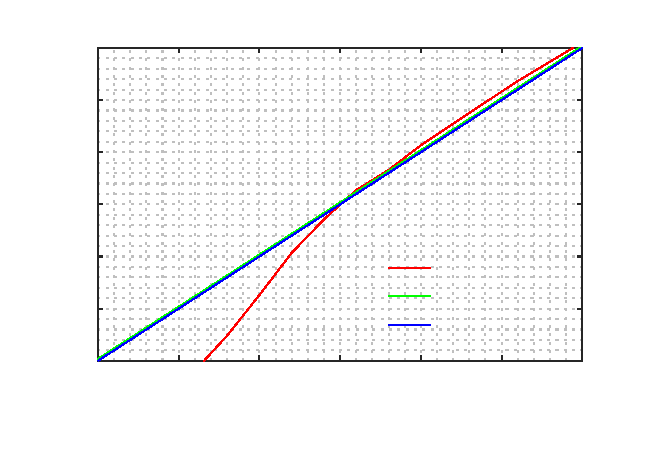
\includegraphics[scale=1]{snr_cnr-inc}
\end{picture}%
\begin{picture}(300,200)(0,0)
\fontsize{10}{0}\selectfont\put(39,27){\makebox(0,0)[t]{\textcolor[rgb]{0.15,0.15,0.15}{{0}}}}
\fontsize{10}{0}\selectfont\put(77.75,27){\makebox(0,0)[t]{\textcolor[rgb]{0.15,0.15,0.15}{{5}}}}
\fontsize{10}{0}\selectfont\put(116.5,27){\makebox(0,0)[t]{\textcolor[rgb]{0.15,0.15,0.15}{{10}}}}
\fontsize{10}{0}\selectfont\put(155.25,27){\makebox(0,0)[t]{\textcolor[rgb]{0.15,0.15,0.15}{{15}}}}
\fontsize{10}{0}\selectfont\put(194,27){\makebox(0,0)[t]{\textcolor[rgb]{0.15,0.15,0.15}{{20}}}}
\fontsize{10}{0}\selectfont\put(232.75,27){\makebox(0,0)[t]{\textcolor[rgb]{0.15,0.15,0.15}{{25}}}}
\fontsize{10}{0}\selectfont\put(271.5,27){\makebox(0,0)[t]{\textcolor[rgb]{0.15,0.15,0.15}{{30}}}}
\fontsize{10}{0}\selectfont\put(33.8008,34.8252){\makebox(0,0)[r]{\textcolor[rgb]{0.15,0.15,0.15}{{0}}}}
\fontsize{10}{0}\selectfont\put(33.8008,59.854){\makebox(0,0)[r]{\textcolor[rgb]{0.15,0.15,0.15}{{5}}}}
\fontsize{10}{0}\selectfont\put(33.8008,84.8833){\makebox(0,0)[r]{\textcolor[rgb]{0.15,0.15,0.15}{{10}}}}
\fontsize{10}{0}\selectfont\put(33.8008,109.913){\makebox(0,0)[r]{\textcolor[rgb]{0.15,0.15,0.15}{{15}}}}
\fontsize{10}{0}\selectfont\put(33.8008,134.942){\makebox(0,0)[r]{\textcolor[rgb]{0.15,0.15,0.15}{{20}}}}
\fontsize{10}{0}\selectfont\put(33.8008,159.971){\makebox(0,0)[r]{\textcolor[rgb]{0.15,0.15,0.15}{{25}}}}
\fontsize{10}{0}\selectfont\put(33.8008,185){\makebox(0,0)[r]{\textcolor[rgb]{0.15,0.15,0.15}{{30}}}}
\fontsize{11}{0}\selectfont\put(155.25,13){\makebox(0,0)[t]{\textcolor[rgb]{0.15,0.15,0.15}{{FM demod input CNR (dB)}}}}
\fontsize{11}{0}\selectfont\put(16.8008,109.913){\rotatebox{90}{\makebox(0,0)[b]{\textcolor[rgb]{0.15,0.15,0.15}{{FM demod output SNR (dB)}}}}}
\fontsize{9}{0}\selectfont\put(202.505,79.3164){\makebox(0,0)[l]{\textcolor[rgb]{0,0,0}{{FM Simulated}}}}
\fontsize{9}{0}\selectfont\put(202.505,65.8179){\makebox(0,0)[l]{\textcolor[rgb]{0,0,0}{{FM Theory}}}}
\fontsize{9}{0}\selectfont\put(202.505,51.8198){\makebox(0,0)[l]{\textcolor[rgb]{0,0,0}{{ SSB Theory}}}}
\end{picture}

\end{center}
\end{figure}


TODO: different threshold expressions based on CNR definition. Independence of CNR

TODO: Tibors measurements

\bibliographystyle{plain}
\bibliography{fm_snr_refs}
\end{document}
